\documentclass[a4paper,11pt,twoside]{book}
\usepackage{listings}		
\usepackage{graphicx}
\usepackage[dvipsnames]{xcolor}
\usepackage{multicol}
\usepackage{amsmath}
\setlength{\emergencystretch}{10pt}
\graphicspath{ {./img/} }	
% \pagecolor{Periwinkle}
% \color{purple}				

\lstset{language=Java,						
	showspaces=false,
	showtabs=false,
	breaklines=true,
	showstringspaces=false,
	breakatwhitespace=true,
	commentstyle=\color{ForestGreen},
	keywordstyle=\color{blue},
	stringstyle=\color{red},
	identifierstyle=\color{Gray},
	basicstyle=\small\ttfamily
}

\begin{document}

\title{Appunti di Reti di Calcolatori}
\author{Simone Ianniciello}
\date{A.A. 2020/2021}
\maketitle

\tableofcontents

\chapter{Introduzione alle Reti}

\section{Introduzione}

\paragraph{Rete}

Con rete si intende un'interconnessione di dispositivi in grado di scambiarsi informazioni.
Le reti sono commposte da elementi quali:
\begin{itemize}
    \item Sistemi terminali \textit{(Host)}
    \subitem Macchine degli utenti finali
    \subitem Server \textit{Fornitori di servizi}
    \item Switch: Dispositivi adibiti all'interconnessione locale di Host
    \item Router: Dispositivi di interconnessione di reti diverse
    \item Collegamenti: I mezzi tramite i quali vengono trasferite le informazioni
    \subitem Cavi in rame
    \subitem Fibra ottica
    \subitem Onde radio \textit{(WiFi)}
\end{itemize}

\section{Tipi di rete}
\paragraph{LAN}
Con \textit{LocalAreaNetwork} o \textit{Rete Locale} si intende un insieme di Host appartenenti allo stesso ente \textit{(Organizzazione, Casa, Scuola)} in grado di comunicare.\newline
Le LAN possono essere:
\begin{itemize}
    \item a cavo condiviso: Tutti gli host condividono lo stesso cavo per comunicare.
    Questo sistema non e' piu' usato perche' poco efficente.
    \item con switch: Tutti gli host sono collegati a uno switch che instrada le informazioni nella direzione desiderata.
    Questo sistema e' molto piu' efficiente perche' le macchine non hanno bisogno di monopolizzare la rete.
\end{itemize}
\paragraph{WAN}
Per \textit{WideAreaNetwork} o \textit{Rete Geografica} si intende una rete formata da piu' LAN e/o singoli host separati da grandi distanze.
Essa viene gestita da da un operatore che fornisce il servizio di interconnessione ai clienti.\newline
Le WAN si distinguono in: 
\begin{itemize}
    \item WAN punto-punto
    \item WAN a commutazione
\end{itemize}
Una applicazione tipica sono reti locali appartenenti ad un'azienda interconnesse tramite WAN p-p
\section{Tecniche di commutazione}
I due sistemi principali per determinare il percorso tra due host e dedicargli le risorse sono:
\begin{itemize}
    \item Circuit-switched network \textit{(Commutazione di circuto)}
    \item Packet-switched network \textit{(Commutazione di pacchetto)}
\end{itemize}
\paragraph{Commutazione di circuito}
Per la commutazione di circuito si procede instaurando un cammino dedicato tra i due host: vengono assegnate le risorse necessarie alla comunicazione e sono garantite per l'intera durata della connessione.
Cio' significa che una volta instaurata la connessione, essa non verra' disturbata in alcun modo.\newline
I principali problemi di questa tecnica sono pero' il tempo di instaurazione della connessione \textit{(risorse non disponibili)}, e il non sfruttamento delle risiorse disponibili durante i \textit{silenzi} nella comunicazione.
\paragraph{Commutazione di pacchetto}
Nelle connessioni a commutazione di pacchetto il flusso di dati viene diviso in pacchetti ed essi vengono \textit{spediti sulla rete} sul percorso prescelto.
Le risorse vengono quindi utilizzate solo se necessarie e possono essere condivise da pacchetti provenienti da host differenti.

Ogni nodo della rete si occupa di ricevere e riservire i pacchetti che gli arrivano. Per fare cio' il commutatore, dopo aver ricevuto un pacchetto, lo mette in una coda di tipo FIFO; quando e' pronto a ritrasmettere preleva il primo pacchetto dalla coda.
Cio' porta a dei ritardi (Il commutatore deve ricevere l'intero pacchetto per reinviarlo, i pacchetti potrebbero dover \textit{aspettare} in coda) e a delle perdite di pacchetti (coda piena).\newline
Questo metodo si chiama \textbf{Store and Forward}.
\section{Internet}
Con \textbf{i}nternet si intende un sistema formato da due o piu' reti comunicanti.
L'\textbf{I}nternet e' l'insieme di reti piu' comune. Ogni rete che intende aggiungersi ad essa deve seguire L'Internet Protocol (IP) e rispettare certe convenzioni.

L'infrastruttura di Internet fornisce servizi di comunicazione alle applicazioni
\begin{itemize}
    \item Senza connesione \textbf{(UDP)}
    \item Orientati alla connessione \textbf{(TCP)}
\end{itemize}

Sono stati definiti dei \textbf{protocolli} di comunicazione per le applicazioni piu' comuni di Internet \textit{(TCP, IP, HTTP, FTP...)}

Ci sono delle organizzazioni adibite alla definizione degli standard di internet:
\begin{itemize}
    \item \textbf{IETF} Internet Engineering Task Force
    \begin{itemize}
        \item Studia e sviluppa i protocolli in uso su internet.
        \item Pubblica i documenti ufficiali che li descrivono sotto forma di RFC/STD \textit{(Request For Comments, STanDards)}
    \end{itemize}
    \item \textbf{ICANN} Internet Corporation for Assigned Names and Numbers
    \begin{itemize}
        \item Coordina i DNS
        \item Assegna i gruppi di indirizzi di rete
        \item Ha funzioni di controllo semplice dello sviluppo di Internet
    \end{itemize}
    \item \textbf{W3C} World Wide Web Consortium
    \begin{itemize}
        \item Sviluppa di standard aperti \textit{(HTML, XML...)}
    \end{itemize}
\end{itemize}

\subsection{Strati della rete}
Le reti degli host si collegano a Internet tramite gli ISPs \textit{Internet Service Provider}.
I livelli della rete sono:
\begin{description}
    \item[Livello 3] ISP di accesso: Sono quelli a cui si connettono comunemente le reti locali.
    \item[Livello 2] ISP regionali: Sono dei collegamenti intermedi che uniscono tutti gli ISP di livello 2 in una zona geografica
    \item[Livello 1] Dorsali: Esse sono la parte piu' \textit{alta} di Internet, tutti gli altri ISP si connettono ad esse. \textit{(ne esistono circa 11)}
\end{description}

\subsection{Peering point}
Sono accordi tra due ISP che gli permettono di ricevere e riinoltrare il traffico da uno all'altro:
per fare cio' esistono gli IXP \textit{(Internet eXchange Point)} ovvero sistemi, anche gestiti da aziende di terzi, che effettuano il peering.
\subsection{Reti di acesso}
Il collegamento tra l'utente e Internet e' detto \textbf{rete di accesso}.
\begin{itemize}
    \item Accesso via rete telefonica
    \begin{itemize}
        \item dial-up
        \item Digital Subscriber Line \textbf{(DSL)}
        \item Fibra ottica
    \end{itemize}
    \item Accesso tramite reti wireless
    \begin{itemize}
        \item 3G, 4G, 5G
    \end{itemize}
    \item Collegamento diretto
    \begin{itemize}
        \item Collegamenti WAN dedicati per aziende, universita'...
    \end{itemize}
\end{itemize}
\newpage
\section{Metriche di riferimento}

\paragraph{Larghezza di banda (Bandwidth)}
Larghezza in Hertz dell'intervallo di frequenze utilizzato per la trasmissione.
\paragraph{Velocita' di trasmissione (bitrate)}
Quantita' di dati trasmissibili nell'unita' di tempo (bps).
\paragraph{Troughput}
Quantita' di dati trasmissibili da un nodo A ad un nodo B in una unita' di tempo.
Tiene di conto anche di perdite sulla rete, protocolli, ecc\dots
\paragraph{Latenza}
Tempo che intercorre tra l'invio e la ricezione del primo bit di un messaggio.
\begin{quote}
    \small Latenza = elaborazione + accodamento + trasmissione + propagazione
\end{quote}
\subsection{Ritardi}
\paragraph{Ritardo di elaborazione}
Causato dal sistema di controllo degli errori e dal sistema che determina il canale di uscita.
\paragraph{Ritardo di accodamento}
Tempo tra l'inserimento nella coda di trasmissione e la ritrasmissione del pacchetto.
\paragraph{Ritardo di trasmissione}
Tempo impiegato per trasmettere un pacchetto sul mezzo di trasmissione.
\begin{quote}
    Misurato in PacketLenght / BitRate
\end{quote}
\paragraph{Ritardo di propagazione}
Tempo che inpiega un bit ad essere propagato da un nodo all'altro.
\begin{quote}
    Misurato in LinkLenght / PropSpeed $(3-2*10^-8)$
\end{quote}
\paragraph{Ritardo end-to-end}
Ritardo cumulato tra tutti i nodi in una trasmissione. E' pari alla sommatoria dei ritardi tra i vari nodi del collegamento.
\subsection{Prodotto rate-ritardo}
Numero massimo di bit che possono \textit{essere contenuti} nel mezzo trasmissivo.
\newpage 
\section{Modelli stratificati}
Il modello statificato permette di scomporre un sistema complesso in piu' sistemi piu' facili da implementare e comprendere.
La modularizzazione dei livelli permette di dividere l'interfaccia dall'implementazione di un servizio.
Percio' dall'esterno ogni modulo e' visto come un'interfaccia che: accetta determinati parametri in ingresso, esegue le sue mansioni, e ritorna una risposta.
Quindi l'implementazione puo' essere cambiata senza che il resto del sistema \textit{ne venga a conoscenza}
\section{OSI RM \small(Open System Interconnection Reference Model)}
Nel 1976 sono iniziati i lavori per definire uno standard aperto per i protocolli di Internet.
La ISO ha da prima pubblicato questi standard sotto forma del OSI-RM, che poi e' diventato uno standar internazionale nel 1983 (ISO 7498).

Il modello ISO/OSI prevede la statificazione del protocollo di telecomunicazione.

\paragraph{Gli strati OSI sono:}
\begin{description}
    \item[7] Applicazione - elaborazione dati
    \item[6] Presentazione - unificazione dati 
    \item[5] Sessione - controllo del dialogo
    \item[4] Trasporto - trasferimento dati tra hosts
    \item[3] Rete - instradamento del traffico
    \item[2] Datalink - consegne trame sul link
    \item[1] Fisico - trasmette un flusso di bit
\end{description}
Le informazioni si propagano dal livello piu' alto (applicazione) fino al piu' basso per poi passare sul mezzo trasmissivo e risalire i livelli fino alla destinazione.

Ogni livello aggiunge all'informazione del livello superione una propria sezione informativa (header / trailer)
Questo processo di incapsulamento delle informazioni e' reversibile percio' ogni livello e' in grado di estrarre i dati degli strati superiori.

\section{Stack Protocollare TCP-IP}
E' la famiglia di protocolli attualmente utilizzata in Internet.
E' definita attualmente da cinque livelli:
\begin{description}
    \item[Applicazione] Applicazioni di rete, collegamento logico end-to-end, scambio di messaggi tra processi. \textit{\tiny ftp, smtp, http}
    \item[Trasporto] Trasferimento dati end-to-end. \textit{\tiny tcp, udp}
    \item[rete] Instradamento dei datagrammi. \textit{\tiny IP, ICMP}
    \item[Link] Trasferimento dei dati in frame tra elementi vicini. \textit{\tiny ppp, ethernet, \dots} 
    \item[Fisico] Trasferimento di bit di un frame sul mezzo trasmissivo. 
\end{description}
\chapter{Lo Strato Applicativo: URI-HTTP}
\section{Applicazioni di rete}
Sono applicazioni formate da processi distibuiti comunicanti; Cio' significa che i processi possono essere eseguiti su host diversi sulla rete.
Sullo stesso host piu' processi possono comunicare anche attraverso la {\color{blue}comunicazione inter-processo} definita dal sistema operativo (quindi esterna alla rete).
Due processi su macchine diverse comunicano tramite la rete con dei \textbf{\color{blue} messaggi}.
Grazie alla statificazione dei livelli, i livelli applicazione comunicano tra loro come se esistesse un collegamento diretto tra i due.
\section{Protocollo dello Strato di Applicazione}
Esso definisce:
\begin{itemize}
    \item i tipi di messaggi scambiati
    \item la sintassi dei messaggi \textit{(i campi)}
    \item la semantica dei campi \textit{(il significato)}
    \item le regole per l'invio dei messaggi \textit{(quando e come)}
\end{itemize}
\newpage
\section{Paradigmi}
\begin{description}
    \item[Client-Server] I server \textit{(pochi ma potenti)} offrono un servizio e sono sempre in attesa di richieste.
    \item[Peer-tp-Peer (p2p)]  I peer offrono e richiedono servizi contemporaneamente.
    \item[Misto] Programmi che utilizzano entrambi i paradigmi per utilizzi diversi \textit{(Skype, \dots)} 
\end{description}
\section{Application Programming Interface (API)}
E' un insieme di regole da rispettare per utilizzare le risorse di un servizio.
Per esempio, se un processo vuole inviare un messaggio sulla rete, utilizza delle chiamate al sistema operativo che comunica con gli strati inferiori dello stack TCP-IP attraverso l'{\color{blue}Interfaccia Socket}.
\paragraph{L'Interfaccia Socket} E' un'API che collega gli strati applicazione e trasporto.
Grazie ad essa un programmatore che intende sviluppare un'applicazione con accesso a Internet non deve preoccuparsi di tutte le \textit{formalita'} per la connessione.
Per identificare un processo sulla rete si utilizza una coppia:
\begin{center}
    \textbf{\color{blue} $<$Indirizzo IP (32b) + numero di porta (16b)$>$}
\end{center}
\section{Uso dei servizi di trasporto}
Nel livello di trasporto sono previsti dule protocolli principali:
\begin{description}
    \item[TCP] connection-oriented: client e server devono \textit{salutarsi} prima di iniziare a comunicare; c'e' controllo degli errori sui messaggi.
    \item[UDP] connection-less: \textbf{\huge\color{red}CHAOS!} Non c'e' nessun controllo, il mittente tira i messaggi sulla rete e suppone che il destinatario lo riceva.
\end{description}
UDP e' utile se si ha bisogno di un alto troughput e/o un basso ritardo, ma solo se non ci interessa un trasferimento affidabile al 100\% dei dati \textit{(streaming, videogiochi, \dots)}.
\newpage
\section{Web e HTTP}
\subsection{Il Web}
Una pagina Web consiste di:
\begin{itemize}
    \item Un file HTML
    \item Diversi oggetti referenziati indirizzabili tramite una URL (Uniform Reference Locator)
\end{itemize}
\subsection{Uniform Resource Identifier}
E' una forma generale per identificare una risorsa sulla rete.
Ci sono due tipi di URI:
\begin{description}
    \item[Uniform Resource Locator (URL)] Risorse identificate tramite il meccanismo di accesso \textit{(HTTP, FTP, \dots)}
    \item[Uniform Resource Name (URN)] Identificatore globalmente unico, anche se la risorsa diventa non disponibile.
\end{description}
\subsection{Sintassi URL}
\begin{center}
    \color{blue}\textit{scheme://host:port/path}
\end{center}
\begin{itemize}
    \item scheme: protocollo di accesso
    \item host: nome di dominio o indirizzo IP
    \item port: numero di porta del servizio richiesto
    \item path: identifica la risorsa nel contesto sopra-descritto
\end{itemize}
Nelle URL HTTP si aggiunge anche un parametro \textit{\color{blue}?query} dopo \textit{\color{blue}path}.
Questa stringa viene interpretata dal server e serve a passare informazioni aggiuntive nella richiesta.
\subsection{URI Assolute e Relative}
\begin{description}
    \item[URI assoluta] identifica una risorsa indipendendentemente dal contesto.
    \item[URI relativa] identifica una risorsa in relazione ad un'altra URL e viene interpretata dal client prima di mandare la richiesta. 
\end{description}
\section{HyperText Transfer Protocol (HTTP)}
Protocollo {\color{blue} stateless} pubblicato nel 1990 e utilizzato fino ad ora nel World Wide Web.
Una caratteristica fondamentale dell'HTTP e' la tipizzazione e negoziazione della rappresentazione dei dati percio' non e' limitato all'ipertesto.

Il client stabilisce una connessione e invia richieste ({\color{blue}request}) tramite HTTP al server, il quale invia messaggi di risposta ({\color{blue}response})
Usa TCP dato che il trasferimento deve essere senza perdite e che i ritardi non sono \textit{un problema}

Dalla versione 1.1 la connessione client-server, a meno che diversamente espresso dal client, e' persistente; percio' il client puo' assumere che il server manterra' la connessione aperta.
Cio' porta a minor utilizzo di CPU e ritardi minori dato che non c'e' bisogno di riaprire una nuova connessione per ogni richiesta.
Inoltre si ha un mignor controllo di congestione.

La connessione viene chiusa dal server solo quando esplicitamente richiesto dal client nell'header del messaggio, o se non riceve piu' richieste (time out)

% \subsection{Pipelining e HeadOfLineBlocking}

% Per migliorare le le prestazioni il client puo' inviare contemporaneamente piu' richieste al server, il quale \textbf{DEVE} rispondere nello stesso ordine in cui sono state ricevute.

% Se pero' una richiesta richiede piu' tempo al server per essere processata blocca tutte le risposte successive e porta all'HOLB. In questi casi non si ha un miglioramento delle performance.

% \newpage
\subsection{HTTP Request}

La richesta e' formata da:
\begin{quote}
    Request-Line \\
    *( general-header \\
    $\vert$ request-header \\
    $\vert$ entity-header ) \\
    CRLF \\
    $[$ message-body $]$
\end{quote}

\subsection{HTTP Response}

La risposta e' formata da:
\begin{quote}
    Status-Line \\
    *( general-header \\
    $\vert$ response-header \\
    $\vert$ entity-header ) \\
    CRLF \\
    $[$ message-body $]$
\end{quote}

\paragraph{Request-Line}
\begin{quote}
    Method SP \\
    Request-URI SP \\
    HTTP-Version CRLF
\end{quote}
\paragraph{Status-Line}
\begin{quote}
    HTTP-Version SP \\
    Status-Code SP \\
    Reason-Phrase CRLF
\end{quote}
\paragraph{General-header} Relativi alla connessione.
\paragraph{Entity-header} Relativi all'entita' trasmessa.
\paragraph{Request-header} Relativi alla richiesta.
\paragraph{Response-header} Nel messaggio di risposta.
\subsection{Content Negotiation}
Le risorse possono essere disponibili in piu' rappresentazioni; Il client puo' richiederne una in particolare tramite richieste su Request e Entity headers.
\subsection{Request methods}
\paragraph{OPTIONS} Il server ritorna solo le opzioni di comunicazione associate ad una URL (capacita', metodi esposti, \dots).
\paragraph{GET} Richiede il trasferimento della risorsa indicata. Sono possibili i \textbf{conditional-get} (If-Mofidied-Since, If-Match, \dots).
\paragraph{HEAD} Simile alla GET ma il server non trasferisce il message-body. Utile per controllare lo stato dei documenti (validita', modifiche, \dots).
\paragraph{POST} Serve per inviare al server informazioni inserite nel body del messaggio.
\paragraph{PUT} Chiede al server di creare/modificare una risorsa (Recuperabile poi tramite GET).
\paragraph{DELETE} Il client chiede di eliminare una risorsa identidficata dalla Request-URI.
\subsection{Caching}
E' possibile memorizzare copie temporanee di risorse Web e ri-servirle al client senza contattare il server.
Si possono avere:
\begin{description}
    \item[User-Agent Cache] Risorsa mantenuta dal browser.
    \item[Proxy Cache] Il proxy mantiene una copia delle risorse richieste. Quando un browser richiede una risorsa cached essa gli viene riservita dal proxy senza interrogare nuovamente il server.
\end{description}
\subsection{Cookies}
Essendo stateless, non e' mantenere una memora su un'applicazione web (come ad esempio l'identita' di un client).
Una soluzione e' utilizzare i cookies, cioe' id unici che il client presenta al server ogni volta che esso effettua una richiesta.

Alla prima connessione, il server invia la normale risposta HTTP + una line \textbf{Set-cookie: id}.
Il client si salva il cookie e lo associa al server. Ogni successiva richiesta a quel server conterra' quel cookie.

\section{Versioni HTTP}
\paragraph{HTTP/1.1}
Permette di instaurare piu' connessioni contemporaneamente perciò il client puo' inviare piu' richieste al server contemporaneamente \bluetext{(Pipelining)}.

Il server deve pero' rispondere nello stesso ordine in cui sono arrivate le richieste perciò, se una richiesta richiede piu' tempo per essere elaborata, tutte le risposte successive non possono essere inviate \bluetext{(HeadOfLineBlocking)}.
\paragraph{HTTP/2}
Aggiunge caratteristiche allo standard HTTP come:
\begin{itemize}
    \item Multiplexing delle richieste su un'unica connessione TCP attraverso la definizione di:
    \begin{description}
        \item[Frame] Un messaggio HTTP viene mappato da una sequenza di Frame (come Data Frame, Headers Frame, \dots).
        \item[Stream] E' un flusso bidirezionale di frame all'interno di una connessione TCP; mediante l'astrazione di essi, e' possibile effettuare il multiplexing delle richieste (piu' stream su un'unica connessione). E' possibile anche associargli un peso (priorità), e una dipendenza verso altri stream.
    \end{description}
    \item Compressione delle intestazioni.
    \item Server Push (permette al server di inviare risorse aggiuntive oltre a quella richiesta dal client).
\end{itemize}
\paragraph{HTTP/3}
E' un'evoluzione di HTTP/2 che usa i servizi di QUIC, un protocollo di trasporto basato su UDP. QUIC aggiunge controllo del flusso e della congestione, e rilevazione dell'errore e delle perdite. Grazie all'astrazione dello stream a livello di trasporto, il rallentamento o la perdita di uno di essi non influisce sugli altri.

\chapter{Lo Strato Applicativo: Telnet}
TErminaL NETwork e' un protocollo che permette l'uso di shell su macchine remote.
Permette al client di effettuare una sessione di login al server, dopo la quale esso puo' accedere a comandi e programmi disponibili sulla macchina remota.

Dopo il login, vengono passate le battute dei tasti al server come standard-input e l'output viene riportato direttamente al client.

Il protocollo TELNET [RFC854] detta che:
\begin{itemize}
    \item Il client stabilisce una connessione di tipo TCP (tipicamente sulla porta 23) con il server. la connessione persiste per tutta la durata della sessione di login.
    \item Vengono \textit{"collegate"} le STDIN e STDOUT dei tue terminali.
\end{itemize}
Il server Telnet utilizza uno Pseudo Terminal Driver per eseguire i comandi.
\section{Network Virtual Terminal: NVT}
Telnet deve poter operare con il numero massimo di sistemi quindi deve poter lavorare con client su sistemi operativi diversi.

Per fare questo il client e il server passano attraverso un terminale virtuale in modo da avere una sola codifica ed entrambi effettuano una conversione dalla propria a quella del NVT.
Sulla rete vengono quindi trasferiti i comandi con l'\textbf{NVT Character Set}.
\newpage
\section{NVT Character Set}
I dati vengono trasferiti tramite 7-bit US-ASCII.
\begin{itemize}
    \item Ogni carattere e' inviato come un byte con il primo bit settato a 0.
    \item Per le sequenze di comandi si imposta il bit piu' significativo a 1.
    \item I comandi come EOL iniziano con 0xFF (Interpret As Command \textbf{IET})
\end{itemize}

\chapter{Lo Strato Applicativo: DNS}
\section{Introduzione}

Ogni rete e' identificata sulla rete tramite un indirizzo IP.
Il problema di essi e' che non sono facili da ricordare \textit{\tiny e sono brutti}.
E' quindi nato il bisogno di associare gli IP a dei nomi logici (e spesso mnemonici).
Per associare gli IP ai nomi e' stato creato il DNS.

Il DNS adotta il paradigma client-server.
Si affida al protocollo di trasporto sottostante per trasferire i messaggi.
E' costituito da:
\begin{itemize}
    \item Uno schema di assegnazione dei nomi
    \item Un database distribuito contenente le associazioni 
    \begin{center}
        $nome dominio \implies IP$
    \end{center}
    \item Un protocollo per la distribuzione delle informazioni sui nomi tra i name server
    \begin{itemize}
        \item Utilizza UDP (porta 53) [oppure TCP]
    \end{itemize}
\end{itemize}

\section{Servizi DNS}
\paragraph{Risoluzione} Traduzione $hostname \implies indirizzo IP$
\paragraph{Host aliasing} Traduzione $nomi \implies nome canonico / IP$
\paragraph{Mail server aliasing} Stessa cosa degli host, permette tra le altre cose di usare nomi identici per mail e web server.
\paragraph{Distribuzione di carico} Ad un hostname possono corrispondere piu' indirizzi IP; il DNS restituisce la lista di IP variandone l'ordinamento ogni volta.
\section{Spazio dei nomi}
{\color{YellowOrange}\paragraph{Struttura "flat"} Sequenza di caratteri senza alcuna ulteriore struttura (deprecato)}
\paragraph{Struttura gerarchica} Il nome e' costituito da diverse parti
\begin{center}
    (p.e. studenti.di.unipi.it)
\end{center}
L'assegnazione dei nomi e' delegabile al sistema decentralizzato. 
\subsection{Nomi di dominio}
I nomi hanno una struttura ad albero. Ogni nodo e' individuato da un'etichetta.(la radice ha etichetta vuota)
\newline
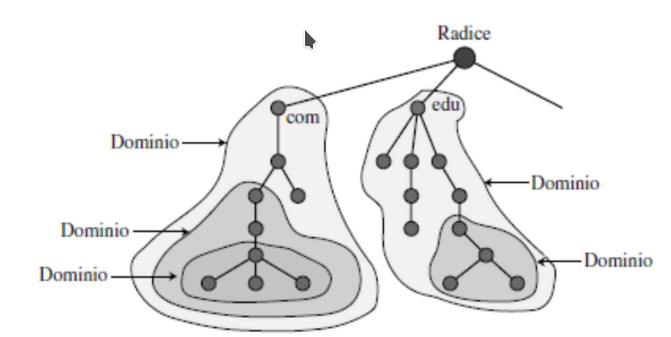
\includegraphics[width=\textwidth]{dns-tree}
La struttura gerarchica permette autonomia nella scelta dei nomi all'interno di un dominio.
\subsection{Esempi di Top Level Domain (TLD)}
\begin{description}
    \item[com] Organizzazioni commerciali
    \item[edu] Istituti di istruzione
    \item[mil] Gruppi militari
    \item[gov] Istituzioni governative
    \item[net] Centri di supporto alla rete
    \item[org] Organizzazioni diverse dalle precedenti
    \item[it, uk, fr, us] Schema geografico per nazioni  
\end{description}
Mantenuti da IANA (Internet Assigned Numbers Authority)
\section{Gerarchia dei Name Server}
\paragraph{DNS} Database distribuito implementato come gerarchia di piu' Name Server.
\paragraph{Name Server} Gestisce le richieste.
Ogni server immagazzina le informazioni relative alla propria zona inclusi i riferimenti ai server dei domini di livello inferiore.
\subsection{Root Name Server}
Restituisce le informazioni sui name server dei TLD. Ce ne sono centinaia in tutto il mondo.
\subsection{TLD Server}
Mantiene le informazioni dei nomi di dominio che appartengono a un TLD; Restituisce le informazioni sui Name Server di competenza dei sotto domini.
\subsection{Authoritative Name Server}
E' l'autorità per una certa zona. Puo' effettuare traduzioni nome $\implies$ indirizzo o inoltrare la richiesta a altri Name Servers.
Sono di due tipi:
\begin{description}
    \item[Server primari] Mantengono il file di zona.
    \item[Server secondari] Ricevono il file di zona e offrono il servizio di traduzione. 
\end{description}
\subsection{Local Name Server}
E' un Name Server mantenuto dagli ISP.
Le query DNS vengono prima rivolte al server locale il quale, in caso non riesca a risolverle, le inoltra alla gerarchia DNS.
\subsection{Query DNS}
La query puo' essere:
\begin{description}
    \item[Ricorsiva] La richiesta fa il \textit{giro completo} attraversando ogni name server fino a trovare il dominio che sta' cercando.
    \item[Iterativa] Le risposte sono restituite direttamente al client insieme al riferimento al server da contattare.
\end{description}
Se un server supporta le query ricorsive, imposta il bit RA \textit{(Recursion Available)} a true.
Se anche il client imposta il bit BD \textit{(Recursion Desired)} a true, viene effettuata la query in modalità ricorsiva.
\subsection{DNS Caching}
I name server mantengono una memoria delle associazioni gia' richieste, le quali vengono cancellate dopo un tempo di timeout.
\section{Resource Records}
\begin{center}
    RR format: \textbf{(name, value, type, ttl)}
\end{center}
\begin{description}
    \item[TTL] Tempo di vita della risorsa della cache.
    \item[Type] A 
    \begin{description}
        \item[Name]  hostname
        \item[Value] IP 
    \end{description}  
    \item[Type] CNAME
    \begin{description}
        \item[Name] hostname
        \item[Value] nome canonico  
    \end{description} 
    \item[Type] NS
    \begin{description}
        \item[Name] Nome di dominio
        \item[Value] hostname dell'authoritative name server per quel dominio
    \end{description} 
    \item[Type] MX
    \begin{description}
        \item[Name] Nome di dominio
        \item[Value] Nome canonico del server di posta elettronica associato
    \end{description} 
\end{description}
% \subsection{Messaggi DNS} TODO
\textit{\small V. messaggi DNS}

\chapter{Lo Strato Trasporto: Introduzione}
\section{Obbiettivo}
Realizza una comunicazione logica tra processi su terminali diversi.
Cio' significa che essi comunicano come se ci fosse un collegamento diretto tra i due.
Lo strato applicazione trasmette dati allo strato di trasporto, il quale poi comunica con gli strati inferiori per trasmetterli all'host di destinazione.
\section{Servizi offerti}
Lo strato di trasporto si occupa principalmente di multiplexing/demultiplexing e del controllo degli errori.
\subsection{Protocolli}
In base al protocollo utilizzato per la connessione, lo strato di trasporto si occupa anche di altri fattori.
I due protocolli {\tiny(principali?)} sono:
\begin{description}
    \item[TCP] (RFC 793) Si occupa della gestione della connessione, dei controlli di flusso e congestione, e assicura una consegna affidabile.
    \item[UDP] (RFC 768) Protocollo connection-less, non affidabile ma piu' veloce. 
\end{description}
\subsection{Multiplexing/Demultiplexing}
\paragraph{Multiplexing} Lo strato di trasporto si occupa di \textit{accorpare} i flussi di dati e spedirli verso la loro destinazione insieme ad una \textit{busta} di trasporto.
\paragraph{Demultiplexing} Lo strato di trasporto si occupa di ricevere i dati dalla rete e instradarli verso i processi desiderati.
\paragraph{} Entrambi si basano sul socket addres (IP + porta) per identificare i processi.
In base al protocollo usato, lo strato di trasporto si occupa anche del 
\paragraph{Demultiplexing connectionless - UDP}
La \textit{busta} contiene solamente la socket address del destinatario. I datagrammi provenienti da host differenti vengono consegnati tutti alla stessa socket di destinazione.
\paragraph{Demultiplexing orientato alla connessione - TCP}
La \textit{busta} contiene le socket address di mittente e destinatario. Un host puo' supportare piu' socket contemporaneamente (p.e. server Web). Lo strato di trasporto puo' quindi inviare i dati alla socket appropriata in base al mittente.
\subsection{Le porte}
Ogni processo che intende comunicare con la rete (punto di demultiplexing) e' identificato tramite un socket address.
La {\color{blue}porta} e' un valore u-int16(0-65535). 
I range standard sono:
\begin{description}
    \item[System ports] (0-1023) Assegnate da IANA, identificano i processi server.
    \item[User ports] (1024-49151) Assegnate da IANA, non e' possibile la duplicazione.
    \item[Dynamic ports] (49152-65535), Non assegnate da IANA, muoiono al momento della chiusura della connessione.
\end{description}
\subsection{Well known ports}
\begin{tabular}{c c}
        20/tcp & ftp-data \\
        21/tcp & ftp \\
        22/tcp & ssh \\
        23/tcp & telnet \\
        25/tcp & smtp \\
        53/udp & dns \\
        53/tcp & dns \\
        69/udp & tftp \\
        80/tcp & www-http \\
        110/tcp & pop3 \\
        119/tcp & nntp \\
        161/udp & sntp \\
        220/tcp & imap3 \\
        510/udp & RIP \\
        3306/tcp & mysql
\end{tabular}
\chapter{Lo Strato di Trasporto: TCP}
\section{Proprietà del servizio}
I processi effettuano un handshake {\tiny\color{red}COVID!1!}.
Lo strato della connessione risiede sui puni terminali e non sui nodi della rete.

Permette di trasferire un flusso continuo di dati in formato bidirezionale (full-duplex).
Inoltre consente di assegnare una connessione diretta processo - processo.
Offre anche controllo di connessione tramite meccanismi di inizio e fine trasmissione.
Tramite alcuni bit di controllo, permette di correggere alcuni tipi di errore.
Con il controllo di flusso si evita di spedire piu' dati di quanti il destinatario sia in grado di trattare.
Nel caso di sovraccarico della rete, tramite il controllo di congestione, si hanno sistemi di recupero della connessione.
\paragraph{Trasferimento bufferizzato}
Il protocollo TCP puo' suddividere il flusso di byte in segmenti. Per farlo e' necessario un buffer dove immagazzinare i dati finché non ce n'e' un numero sufficiente da essere spediti.
Cio' consente un minor numero di messaggi scambiati per trasferire una sequenza di byte.
\section{Formato dei segmenti}
\subsection{Numeri di sequenza e di riscontro}
\paragraph{Numero di sequenza} e' il numero del primo byte di un segmento.
Generalmente si parte da un Initial Sequence Number (ISN) casuale.
\paragraph{Numero di riscontro} e' il +1 del numero dell'ultimo byte ricevuto correttamente.

\textit{ACK=x} = significa: ho ricevuto tutti i byte fino a \textit{x-1}, aspetto \textit{x}.
\subsection{Forma dei segmenti}
L'header aggiunto al messaggio contiene:
\begin{description}
    \item[Porta sorgente] 16bit
    \item[Porta destinazione] 16bit
    \item[n-SEQ] Numero di sequenza, 32 bit
    \item[n-ACK] Numero di riscontro, 32 bit
    \item[HLEN] Lunghezza dell'header espressa in parole da 4Byte, 4bit
    \item[Reserved] 6bit
    \item[URG] Il campo puntatore contiene i dati da trasferire in via prioritaria, 1bit
    \item[ACK] Considerare n-ACK, 1bit
    \item[PSH] Trasferimento immediato da trasporto a applicazione
    \item[RST] Reset della connessione
    \item[SYN] Sincronizza n-SEQ
    \item[FIN] Chiusura della connessione   
    \item[Dimensione finestra] Numero di byte {\tiny a partire da n-ACK}, elaborabili, 16bit
    \item[Checksum] Considera l'intero pacchetto; serve a rilevare gli errori, 16bit
    \item[Puntatore urgente] {\small Punta al primo Byte non URG partendo da n-SEQ}, 16bit
    \item[Opzioni e riempimento] {\small Negoziazione di vari parametri opzionali}, 0-40Byte
\end{description}
\newpage
\section{Gestione della connessione}
\subsection{Handshake a tre vie}
\begin{description}
    \item[Richiesta di connessione] Il client invia una richiesta al server con:
    \begin{description}
        \item[SYN] 1
        \item[n-SEQ] \#rand {\tiny = x}
    \end{description}
    Il server inizializza due buffer e le variabili di connessione per il controllo di flusso e congestione.
    \item[Autorizzazzione connessione (SYNACK)] Il server risponde con:
    \begin{description}
        \item[SYN] 1
        \item[ACK] 1 
        \item[n-SEQ] \#rand {\tiny = y}
        \item[n-ACK] x+1
    \end{description}
    Il client inizializza gli stessi buffer e variabili.
    \item[ACK] Riscontro positivo dell'avvenuta connessione, contiene:
    \begin{description}
        \item[SYN] 0
        \item[ACK] 1
        \item[n-SEQ] x+1
        \item[n-ACK] y+1 
    \end{description}
    Connessione stabilita.
\end{description}
\subsection{Chiusura della connessione}
\setlength{\columnseprule}{0.4pt}
\setlength{\columnsep}{5em}
\begin{multicols}{2}
    \begin{description}
        \item[C$\implies$S] Chiusura da parte\\del client:
        \begin{description}
            \item[FIN] 1
            \item[n-SEQ] x  
        \end{description} 
        Il client non puo'\\piu' inviare dati.
        \item[S$\implies$C] ACK di chiusura:
        \begin{description}
            \item[ACK] 1
            \item[n-ACK] x+1  
        \end{description}  
        Il server puo' ancora\\inviare dati, il client no.
        \item[S$\implies$C] Chiusura da parte\\del server:
        \begin{description}
            \item[FIN] 1
            \item[n-SEQ] y  
        \end{description} 
        Il server aspetta la\\ricevuta di chiusura.
        \item[C$\implies$S] ACK di chiusura.
        \begin{description}
            \item[ACK] 1
            \item[n-ACK] y+1  
        \end{description} 
        Connessione terminata.
    \end{description}
\end{multicols}
\setlength{\columnseprule}{0pt}
\setlength{\columnsep}{1em}
Quando il client riceve FIN dal server entra nello stato {\color{blue} TIME\_WAIT} e ci resta per un tempo dettato da MSL (diverso su macchine differenti) prima di poter chiudere totalmente la connessione. Questo serve nel caso l'ultimo ACK venga perso perché a un certo punto uno dei due host richiederà la chiusura passiva e l'altro dovrà rispondere con un ACK.
Allo stesso modo dell'handshake di apertura, si puo' avere un three-way handshake di chiusura.
\section{Stati TCP}
\subsection{Stati client}
\begin{description}
    \item[SYN-SENT] Dopo aver inviato una richiesta di connessione, si aspetta la conferma.
    \item[ESTABLISHED] La connessione e' pienamente stabilita, e' possibile trasferire dati.
    \item[FIN-WAIT-1] Il client aspetta una richiesta di chiusura o l'ack di una sua richiesta di terminazione.
    \item[FIN-WAIT-2] Aspetta la richiesta di terminazione di connessione da un host remoto. 
    \item[TIME-WAIT] Vedi sopra.
    \item[CLOSED] Connessione chiusa. Non e' piu' possibile comunicare.
\end{description}
\subsection{Stati server}
\begin{description}
    \item[LISTEN] In attesa di una connessione TCP qualunque.
    \item[SYN-RECEIVED] Si entra in questo stato appena si riceve una richiesta di connessione.
    \item[ESTABLISHED] Vedi sopra.
    \item[CLOSE-WAIT] Si aspetta la richiesta di chiusura dal client.
    \item[LAST-ACK] Si aspetta l'ack di chiusura.
    \item[CLOSED] Vedi sopra.
\end{description}
\newpage
\section{Trasferimento di dati affidabile}
\subsection{Esempio Telnet su TCP}
\begin{description}
    \item[C$\implies$S] L'utente digita C
    \begin{description}
        \item[n-SEQ] 42
        \item[n-ACK] 79
        \item[data] "C"   
    \end{description}
    \item[S$\implies$C] ACK per ricevuta di C
    \begin{description}
        \item[n-SEQ] 79
        \item[n-ACK] 43
        \item[data] "C"   
    \end{description}
    \item[S$\implies$C] ACK dell'ACK
    \begin{description}
        \item[n-SEQ] 43
        \item[n-ACK] 80
    \end{description}
\end{description}
Il mittente puo' anche inviare piu' segmenti senza attendere il riscontro (pipelining).
\subsection{Eventi lato mittente}
Lo strato di trasporto riceve i dati dall'applicazione, li incapsula, gia assegna un numero di sequenza, ed avvia un timer di ritrasmissione (RTO).

La ritrasmissione avviene in caso di:
\begin{description}
    \item[Timeout] Non si riceve un ACK prima della scadenza del RTO.
    \item[ACK duplicato] Il mittente riceve tre ACK uguali significa che il segmento successivo a quello e' andato perso. Si ha quindi la {\color{blue}fast retransmission}.  
\end{description}
\subsection{Segmenti fuori sequenza}
Se i dati arrivano fuori sequenza (ordinamento sparso), l'entità TCP destinataria puo' memorizzarli temporaneamente ma il protocollo non specifica che utilizzo farne.

Nelle versioni piu' recenti si implementa SACK, che manda l'ACK dei pacchetti fuori sequenza in OPTIONS.
\subsection{Eventi lato destinatario}
Tutti i segmenti inviati per trasmettere dati includono ACK.
\paragraph{Delayed ACK} Se il destinatario riceve un segmento atteso, puo' ritardare l'invio di ACK di 500ms a meno che non riceva un altro segmento.
\paragraph{Fast retrasmission request}Se il destinatario riceve un segmento fuori sequenza, un duplicato, o un capisce che c'e' un segmento mancante, risponde subito con un ACK indicando il segmento da cui ripartire.
\subsection{Calcolo del timeout}
Il RTO deve essere maggiore del Round Trip Time (RTT) (tempo tra l'invio di un messaggio e la ricevuta dell'ACK).
\begin{quote}
    $eRTT = (1 - \alpha) * eRTT + \alpha * sRTT$
\end{quote}
\begin{description}
    \item[eRTT] RTT stimato, cumulativo su piu' misure.
    \item[sRTT] RTT di un segmento trasmesso con successo.
    \item[\textit{alpha}] $1/8$ (RFC2988)
\end{description}
\begin{quote}
    \small$dRTT = (1 - \beta) * dRTT + \beta * (sRTT - eRTT)$
\end{quote}
\begin{description}
    \item[dRTT] Deviazione di eRTT da sRTT
    \item[\textit{beta}] $1/4$ (RFC2988)
\end{description}
\begin{quote}
    {\boldmath$RTO$} $ = eRTT + 4*dRTT$
\end{quote}
In molte implementazioni dopo un errore si raddoppia RTO
\subsection{Finestra di trasmissione}
Il buffer di invio, si dividono i byte in {\color{blue}finestre}.
La finestra di trasmissione e' la sottosezione del buffer di invio che deve essere spedita con il prossimo messaggio.
Ha dimensione variabile (modificata in base alla condizione della rete) per permettere i controlli di flusso e congestione.
Viene fatta avanzare non appena si riceve l'ACK dell'ultima trasmissione.
\section{Controllo di flusso}
Il destinatario di un messaggio mantiene un buffer di ricezione.
il processo sullo strato applicazione legge i dati da una finestra di ricezione (non necessariamente quando arrivano).
Si intende con {\color{blue}controllo di flusso} la capacità del mittente di evitare di saturare il buffer del destinatario.
Il mittente mantiene una variabile detta {\color{blue}finestra di ricezione} (rwnd) che detta lo spazio disponibile nel buffer ricevente; essa e' passata dal destinatario al mittente tramite il campo window nell'header TCP.
\begin{quote}
    $rwnd = RcvBuffer - (LastByteReceived - LastByteRead)$
\end{quote}
\newpage
Il mittente si assicura che:
\begin{quote}
    $LastByteSent - LastByteAcked < rwnd$
\end{quote}
\begin{quote}
    Se $rwnd = 0$ il mittente lo \textit{richiede} con un segmento sonda da un byte
\end{quote}
\section{Controllo di congestione}
Se si provano a spedire troppi dati su una rete che non puo' supportarli avviene il fenomeno della congestione; cio' puo' provocare:
\begin{itemize}
    \item Lunghi ritardi (accodamenti nei buffer)
    \item Perdita di pacchetti (overflow dei buffer)
\end{itemize}
TCP permette il {\color{blue}controllo di congestione}: se si percepisce uno scarso traffico, viene aumentata la frequenza di invio; altrimenti diminuisce.
\subsection{Algoritmo di controllo}
L'algoritmo utilizzato per regolare la frequenza di invio in funzione della congestione e' costituito da tre fasi:
\begin{itemize}
    \item Slow start
    \item AIMD 
    \item Fast recovery
\end{itemize}
\subsection{Finestra di congestione (Congestion Window)}
Misurata in Max Segment Size (MSS); E' il numero di segmenti che si possono inviare insieme, senza bisogno di aspettarne l'ACK. %TODO: Ricontrolla sta roba cretino, tanto non hai capito sicuramente un cazzo
\subsection{Slow start}
All'inizio la congestion window (CW) e' posta a 1MSS.
Per ogni ACK, CW viene aumentata di 1MSS. Cio' significa che essa raddoppia per ogni RTT.
\subsection{Additive Increase Multiplicative Decrease}
La CW viene aumentata in modo da avere un incremento pari a 1MSS per ogni RTT;
Cio' significa che per ogni ACK, cwnd = cwnd+1/cwnd.

Ad ogni evento di perdita di ACK la CWND viene dimezzata.
\subsection{TCP RENO}
Viene definita una variabile di threshold alla quale viene assegnato un valore alto;
Finché $cwnd < threshold$, siamo in slow start (cwnd aumenta esponenzialmente).\newline
Non appena $cwnd > theshold$, si entra in AI.
\paragraph{Se ricevo 3 ACK duplicati} entro in fast recovery:
\[ threshold = \dfrac{cwnd}{2} \]
\[ cwnd = threshold + 3MSS \]
Finché continuano ad arrivare ACK duplicati
\[ cwnd = cwnd + 1 \]
Non appena arriva un ACK non duplicato
\[ cwnd = threshold \]
\paragraph{Se perdo un ACK per timeout} entro in slow start:
\[ threshold = \dfrac{cwnd}{2} \]
\[ cwnd = 1MSS \]
\subsection{TCP Tahoe}
Molto simile a RENO ma timeout e 3 ACK duplicati vengono gestiti allo stesso modo (si va in slow start)
\subsection{Throughput}
Indicando con $W$ la dimensione massima raggiunta dalla finestra, il throughput medio e'
\[ Throughput = \dfrac{0,75 \times W}{RTT} \]
\subsection{Equità (fairness)}
In condizioni perfette, $K$ connessioni TCP che passano sullo stesso link di capacita' $R$ bit/s, le connessioni hanno gli stessi valori di $MSS$ e $RTT$; in questo caso ogni connessione trasmette $R/K$ bit/s.
In condizioni reali pero' le connessioni con $RTT$ piu' piccolo (migliori) variano piu' velocemente $congwin$ e raggiungono throughput superiori.

\end{document}